\begin{figure}[htb]

\begin{minipage}[b]{0.48\linewidth}
  \centering
  \centerline{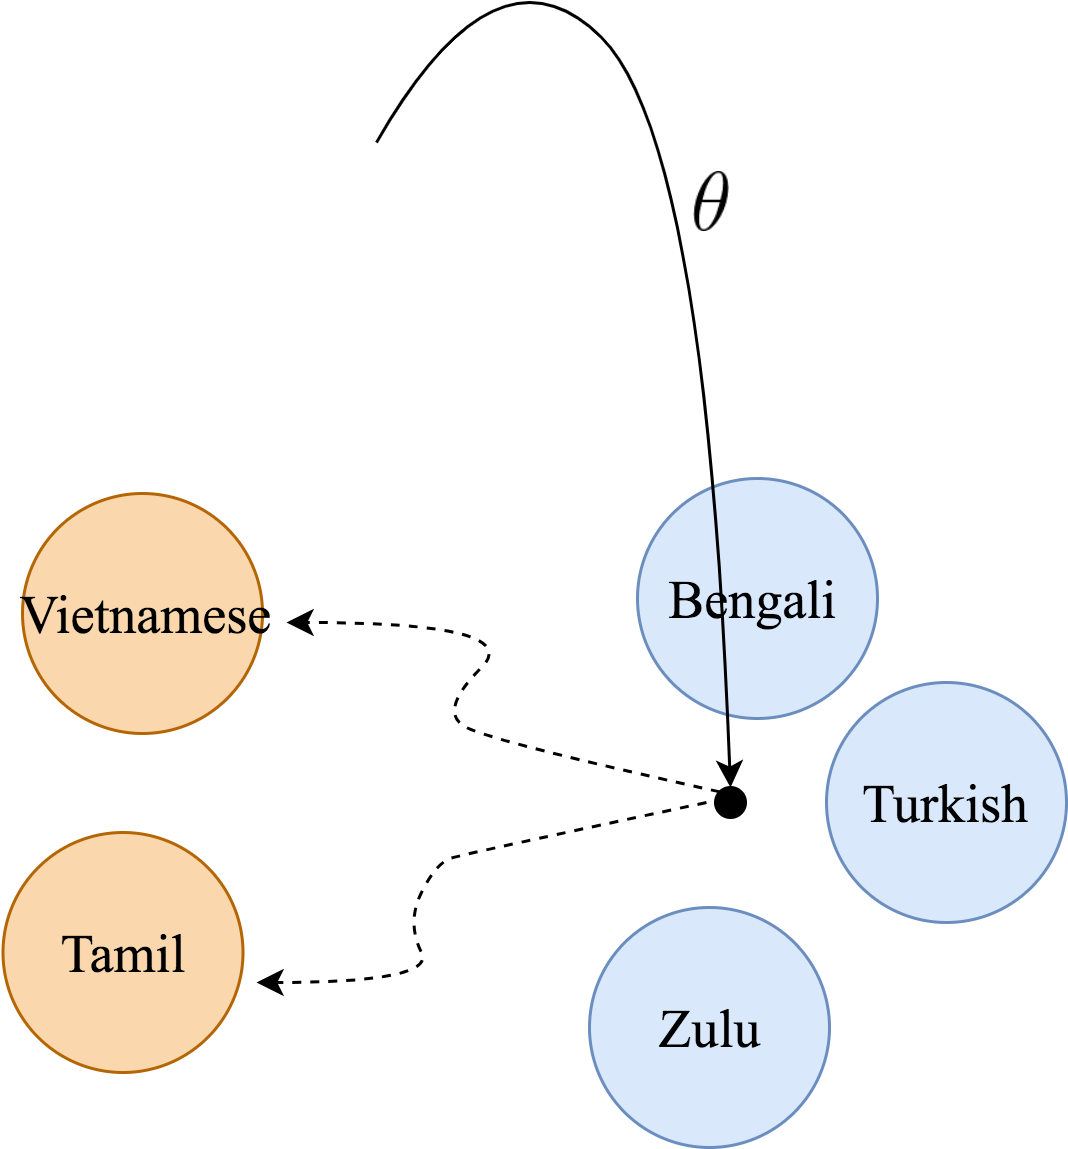
\includegraphics[width=4.0cm]{figs/multi_process.png}}
%  \vspace{1.5cm}
  \centerline{(a) MultiASR}\medskip
\end{minipage}
\hfill
\begin{minipage}[b]{0.48\linewidth}
  \centering
  \centerline{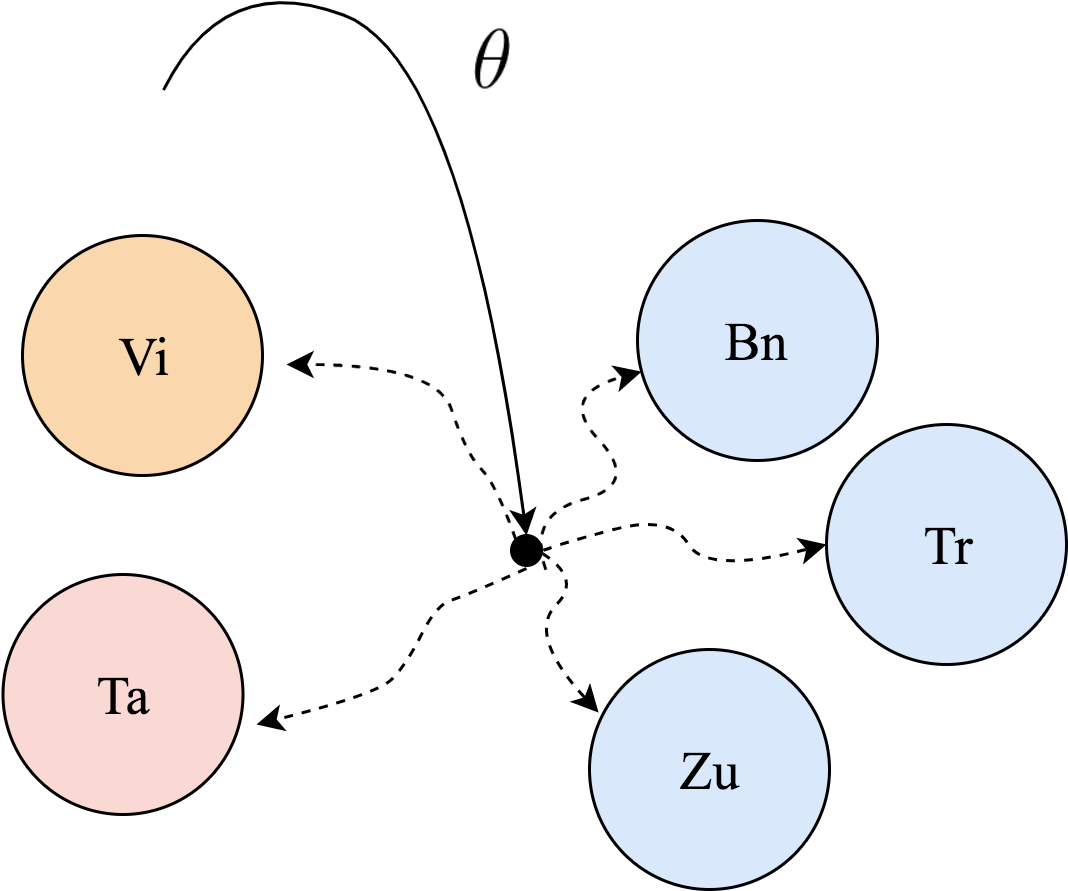
\includegraphics[width=4.0cm]{figs/meta_process.png}}
%  \vspace{1.5cm}
  \centerline{(b) MetaASR}\medskip
\end{minipage}
%
\caption{Illustration: Difference of the learnt parameter from MultiASR \& MetaASR. The solid lines represent the learning process of pretraining, either multitask or meta learning. The dashed lines represent the language-specific adaptation.\\ (The figure is modified from \cite{gu2018meta})}
\label{fig:meta-idea}
%
\end{figure}

